%%
%% 研究報告用スイッチ
%% [techrep]
%%
%% 欧文表記無しのスイッチ(etitle,eabstractは任意)
%% [noauthor]
%%

%\documentclass[submit,techrep]{ipsj}
\documentclass[submit,techrep,noauthor]{ipsj}



% \usepackage[dvips]{graphicx}
\usepackage{latexsym}
\usepackage[dvipdfmx]{graphicx}
\usepackage{tabularx}

\newcommand{\todo}[1]{\colorbox{yellow}{{\bf TODO}:}{\color{red} {\textbf{[#1]}}}}
\newcommand{\ihara}[1]{\colorbox{green}{{\bf IHARA}:}{\color{blue} {\textbf{[#1]}}}}

\def\Underline{\setbox0\hbox\bgroup\let\\\endUnderline}
\def\endUnderline{\vphantom{y}\egroup\smash{\underline{\box0}}\\}
\def\|{\verb|}
%

%\setcounter{巻数}{59}%vol59=2018
%\setcounter{号数}{10}
%\setcounter{page}{1}


\begin{document}


\title{コードレビューにおける\\長期貢献者予測に向けた学習期間の検討}

\affiliate{IPSJ}{和歌山大学\\
Wakayama University}

\author{橋本 一輝}{Hashimoto Kazuki}{IPSJ}[s276189@wakayama-u.ac.jp]
\author{伊原 彰紀}{Ihara Akinori}{IPSJ}[ihara@wakayama-u.ac.jp]


\begin{abstract}
オープンソースソフトウェアプロジェクトの継続的な開発・保守の実現には,長期的に貢献する開発者(長期貢献者)の確保が不可欠であるが,多くの開発者は数回の貢献後に活動が途絶えてしまうことが多い.従来研究では,長期貢献者を早期に特定する研究が進められており,プロジェクト参加後の数ヶ月の貢献に基づいて行われてきたが、コードレビュー作業への継続的な貢献を対象にした研究は進められていない.本研究では、コードレビュー依頼において,逆強化学習(IRL)を用いてレビュアーの貢献を学習し、継続的なタスク受け入れの判断を決定する報酬関数を推定する。
特に、レビュアーがタスクを受け入れる参加確率モデルの予測性能を検証するため、モデルの学習期間と貢献予測期間を動的に変更し、その予測精度と安定性を系統的に調査する。ケーススタディとしてコードレビュー履歴を対象に評価実験を行う.
本研究では,レビュアーの貢献が時間とともにどのように変化し、長期貢献者の予測に最適な学習期間を定量的に分析する。
\end{abstract}


%
%\begin{jkeyword}
%情報処理学会論文誌ジャーナル,\LaTeX,スタイルファイル,べからず集
%\end{jkeyword}
%
%\begin{eabstract}
%This document is a guide to prepare a draft for submitting to IPSJ
%Journal, and the final camera-ready manuscript of a paper to appear in
%IPSJ Journal, using {\LaTeX} and special style files.  Since this
%document itself is produced with the style files, it will help you to
%refer its source file which is distributed with the style files.
%\end{eabstract}
%
%\begin{ekeyword}
%IPSJ Journal, \LaTeX, style files, ``Dos and Dont's'' list
%\end{ekeyword}

\maketitle

%1
\section{はじめに}
オープンソースソフトウェア(OSS)は,世界中のボランティア開発者の貢献によって発展している.これらの貢献者は,営利的な目的ではなく,社会的・技術的など多様な動機に基づき,違いに知識を共有しながら開発を進めてきた.この開発モデルはRaymondが提唱した「伽藍とバザール」における「バザール」モデルに相当する[todo].この開発モデルでは,開発者の多様な参加を促進する一方で,開発者の流動性が極めて高いという課題を抱えている

実際に,開発者の同期は多様であり時間的制約や興味の変化による開発者の離脱も多い.OSSプロジェクトでは多くの開発者が数回の貢献後に活動が停止してしまうことが知られている[todo].こうした開発者の離脱により実際に多くのOSSプロジェクトが失敗している[todo]

プロジェクトの持続可能性を確保する上で重要なのが,プロジェクトに長期的に貢献する長期的貢献者(LTC)の存在である.LTCは単に新しいコードを作成するだけでなく,新規開発者の育成や,ソフトウェアコードレビューといったプロジェクトの中核的な役割を担う.プロセスには十分な知識を要するため,経験が豊富なLTCに作業が集中しやすい[todo].これらの問題を緩和するために,将来のLTC候補となる貢献者を特定し,候補者が離脱しないようサポートを行うことが重要である.

しかし,LTCが担うタスクの1つであるコードレビュー作業への継続的な貢献に着目した研究は十分に進められていない.そこで,本研究では,コードレビュー依頼におけるレビュアーの貢献行動に着目し,IRLを用いて,レビュアーがタスクを受け入れる際の判断指標(報酬関数)を推定し,継続的に貢献するレビュアーを予測するモデルを構築する.特に,モデルの学習期間,予測期間などを変更することにより,予測精度と安定性を調査することで,長期貢献者の予測モデルの検討を行う
\todo{続く2章では,,,3章では,,,,4章では,,,.....}
%3
\section{関連研究}
\subsection{長期貢献者の予測に関して}
ELuriらの研究[todo]では,新規貢献者がプロジェクトに参加した時点で収集が可能な31個の特徴量(コントリビュータに関する特徴量18個,リポジトリの特徴量13個)を用いて,貢献者が3年後も活動があるかどうかを予測するモデルを作成した.予測には5つの機械学習モデルが使用され,その結果Ramdom Forestが最も優れた性能を示し,AUCは0.913であった.彼らが比較対象としたBaoらの研究[todo]も同様に,T年後(T=1 ,2, 3)に貢献者が存在しているかを,プロジェクト参加時点から1ヶ月間の活動から予測する研究であった.
これらの研究は,commitやissue対応といったプロジェクトでの全般的な活動を貢献とみなしている.また,予測においても将来の単一時点での予測に留まっている.
\subsection{開発者の離職予測に関する研究}
開発者の離職を予測する研究も行われいる.例えば,Linらの研究[todo]では,
最初の6ヶ月間の月次レポートに基づき,1年後に離職しているかどうかを予測する機械学習モデルを作成した.その結果,ELuriらの研究と同様にRamdom Forestが最も優れた性能を示し,予測に重要な特徴量としては,月次レポートのタスク報告内容・労働時間の標準偏差・プロジェクトメンバーでの労働時間の標準偏差であった.この研究も同様に,月次レポートに基づく活動でありプロジェクトでの全般的な活動を貢献とみなしている.また,予測に関しても単一の時点である.
\subsection{本研究の位置付け}
2.1及び2.2の従来研究は,コミットや月次レポートといったプロジェクトでの全般的な活動に基づき,単一時点での予測を行っており,LTCや開発者の定着性を予測する上で重要な知見を提供している.
ここで,本研究ではプロジェクトでの全般的な活動ではなく,コードレビュー作業というより専門的な活動に焦点を当て分析する.
また,予測においてもT年後という単一時点の予測から0-3ヶ月後,3-6ヶ月後,6-9ヶ月といった連続的な区間における貢献の有無を予測する.これにより,従来の研究では捉えることができなかった,貢献者が「いつ」活動し,「いつ」離脱するのかといった動的なパターンを捉えることを可能にすることを目的とする.具体的には.また,一度活動を休止した後に再び貢献するといったパターン(例:0-3ヶ月後は活動,3-6ヶ月後は休止,6-9ヶ月後に活動)を特定できる可能性がある.これにより,プロジェクトの管理者が,開発者が「いつ」離脱する可能性が高くなるか,あるいは復帰する可能性があるかを予測することができる.


\label{sec:format}



%4

\label{config}
\section{強化学習・逆強化学習}
本研究では,逆強化学習を使用する.以下で強化学習と合わせて説明する.
\subsection{強化学習}
\begin{figure}[h]
    \centering
    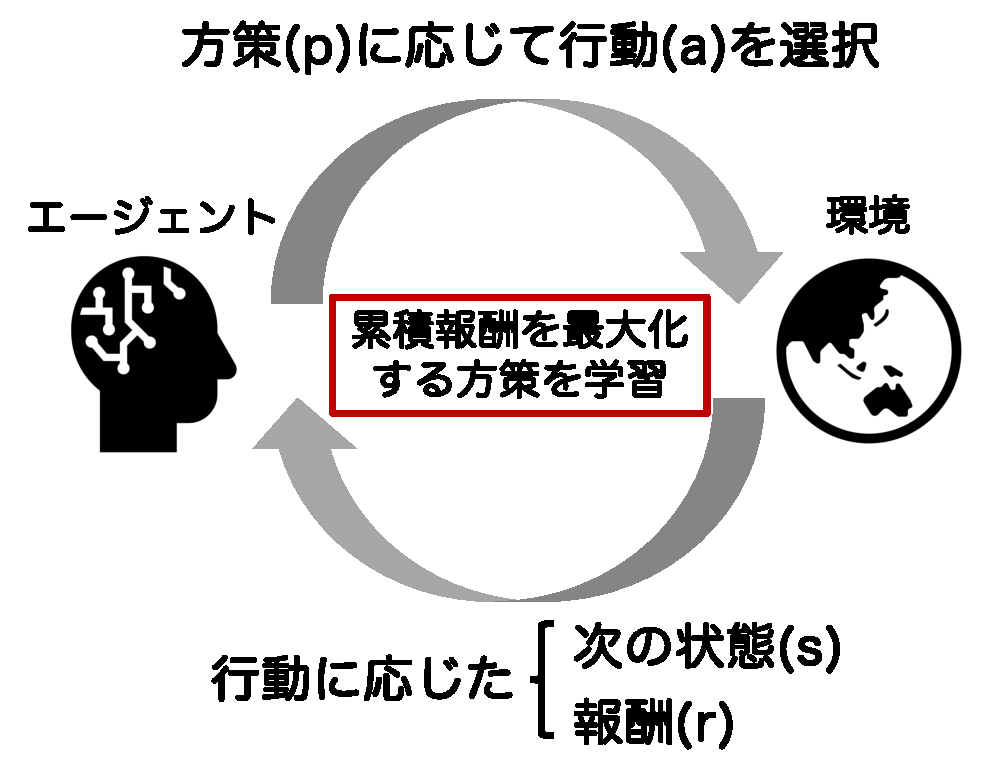
\includegraphics[width=1.0\linewidth]{./Hashimoto_fig/RL.pdf}
    \caption{強化学習のイメージ図}
    \label{fig:RL}
\end{figure}


強化学習(Reinforcement Learning, RL)は,エージェントと環境が相互作用を通じて,累積報酬を最大化するような行動の方策を学習する機械学習の一分野である.以下の基本的な構成要素から成る
\begin{itemize}
    \item エージェント:学習・意思決定を行う主体
    \item 環境:エージェントと相互作用する対象
    \item 状態:環境の現在状況(スナップショット)
    \item 行動:エージェントが取ることの選択肢
    \item 報酬:行動の良し悪しに応じて与えられるスカラー量
    \item 方策:エージェントの行動を決定する
\end{itemize}
強化学習において,報酬関数R(s,a)は最も重要な要素であり,報酬関数が,エージェントの達成するべきことを定義する.しかし,多くの実世界の問題では,複雑や要因が相互に作用しているため,事前に報酬関数を設計することは困難であり,報酬関数が不適切だと意図しない行動を学習してしまう.
\subsection{逆強化学習}
逆強化学習では,強化学習の事前に報酬関数を設計することが困難であるといった課題を解決するために,専門家の行動から,その行動を説明する報酬関数を逆算するアプローチをとる.既知の報酬関数から最適な方策を学習する強化学習に対して,逆強化学習は既知の専門家の軌跡から,その行動を説明する報酬関数を推定する.ここでの専門家の軌跡とは,状態と行動のペアを時系列に並べたものであり,専門家はなんらかの報酬関数(目的)を最大化するよう行動していると仮定し,その報酬関数を推定する.
\subsubsection{逆強化学習の強み}
従来の教師あり学習でのLTC予測では,単一時点でのスナップショットから予測を行うモデルを作成し,予測を行っていたため,過去の文脈の変化のパターンを捉えることが難しい.しかし,逆強化学習は,時系列の活動を軌跡として扱い,各状態と行動から報酬関数を推定するため,過去の行動パターンが将来の行動の予測に影響を与える.そのため従来では捉えることが難しかった,どのような行動パターンが継続につながるのかといった過去の文脈をより正確に捉えることができるため,本研究では逆強化学習を用いる

\todo{逆強化学習図}


\label{sec:format}
%5
\section{長期貢献者予測モデル}
\label{config}
\todo{手法概略図}

\subsection{データ収集}
\subsubsection{データソース}
本研究では,Gerrit REST APIを用いて,gerritからOpenStackプロジェクトのデータを取得した
\subsubsection{収集データ}
\begin{itemize}
    \item レビュー依頼(Change)
    \begin{itemize}
        \item 変更ID,プロジェクト名,作成日時,ステータス,コード変更量(追加/削除)
    \end{itemize}
\end{itemize}
\begin{itemize}
    \item レビュアー情報
    \begin{itemize}
        \item メールアドレス,名前,アサイン日時
    \end{itemize}
\end{itemize}
\begin{itemize}
    \item レビュー活動
    \begin{itemize}
        \item  レビューコメント内容,投票スコア,応答時刻
    \end{itemize}
\end{itemize}

\begin{itemize}
    \item 活動履歴
    \begin{itemize}
        \item  過去活動統計(レビュー回数,レビュー応答率,プロジェクト在籍日数)
    \end{itemize}
\end{itemize}
\begin{itemize}
    \item レビュアーとの相互用
    \begin{itemize}
        \item レビュアーと変更作成者間の過去の相互作用回数??
    \end{itemize}
\end{itemize}

\subsection{データ前処理}
収集したデータから自動化されたbotアカウント(CI/CD等)と判断されるものを除外した.全てのデータをrequest-time(レビュー依頼時刻)でソートし,時系列順に整列した.


\subsection{ラベル付}
本研究では,逆強化学習において,基準点からレビュアーが指定期間内に活動があるかどうかの二値変数でラベル付を行う.
\subsubsection{ラベルの基準点の設定}
レビュアーの活動ごとにラベルを付与すると,ラベルの数が膨大になり,学習時間の増加や,細かすぎるラベル付により類似した状態での学習が増加するため,過学習になる恐れがある.そのため,本研究では各月の末日を基準点とすることで,その月内の全活動に同一のラベルを付与する,これにより月単位での継続パターンを学習し,より一般化された予測モデルの構築を目指す.
\subsubsection{ラベル付のイメージ}
実際のラベル付は次の通りに行う.
\begin{enumerate}
    \item 活動日から活動月を特定する
    \begin{itemize}
        \item 例:2022-01-05 → 2022年1月
    \end{itemize}
    \item その月の最終日を基準点とする
    \begin{itemize}
        \item 例:2022-01-31
    \end{itemize}
    \item 基準点から指定期間の間で将来の活動があるか調べる(指定期間が0-3mの場合)
    \begin{itemize}
        \item 例:2022-01-31から2022-04-31に活動があるか(基準日から指定期間)
    \end{itemize}
    \item 活動があるかを判定
    \begin{itemize}
        \item 活動あり→True, 活動なし→False
    \end{itemize}
        \item その月の全活動に同じラベルを付与する(4)でTrueの場合
    \begin{itemize}
        \item 1月の全活動にTrueラベルを付与
    \end{itemize}
\end{enumerate}

\subsubsection{ラベルの学習時の役割}
このラベルは,逆強化学習の際に単なる過去の事実としてではなく,その時点での状態が,将来の継続とどう関連しているかを学習するための教師信号として機能する.具体的には,Trueのラベルからは,継続したレビュアーの活動から継続を促進する要因を学習し,Falseのラベルからは離脱したレビュアーのパターンから離脱のシグナルを学習することができる.

\subsection{特徴量抽出}
\subsubsection{状態}
\todo{使用する特徴量の説明(表or箇条書き列挙}
\subsubsection{行動}
\todo{特徴量入れる}

\subsection{学習:損失関数と報酬関数の推定}
\todo{図} \\
本研究のモデル学習は主に,目的関数である損失関数の設定と,逆強化学習(IRL)の原理に基づく報酬関数の最適化のプロセスから成る.
\subsubsection{損失関数:Focal Loss}
長期貢献者の予測というタスクにおいて,約8割の開発者が長期貢献者になる前に,離脱してしまうということが知られている[todo],そのため,正例と負例の間で学習データ数に不均衡が生じる.この不均衡問題を対処するために,本研究では,Focal Lossを使用する.
\subsubsection{Focal Lossの定義}
Focal Loss(FL)は,二値クロスエントロピー(BCE)において,クラスの不均衡が生じた際に,容易に分類できる学習ばかりが進み,難しいサンプルの学習にうまく焦点が当たらない問題を解決するために設計された.具体的んは,分類が容易である(正しく予測することができる)サンプルの損失の重みを小さくし,難しいサンプルに焦点が当たるように設計されている
\[\textbf{Binary Cross-Entropy (BCE)}\]
\[
L_{\mathrm{BCE}} = - \frac{1}{N} \sum_{i=1}^{N} \left[ y_i\log(p_i) + (1 - y_i)\log(1 - p_i)\right]
\]
ここで,
\[p_i = \sigma(z_i) = \frac{1}{1 + e^{-z_i}}\]はシグモイド関数であり,\(y_i \in \{0,1\}\) は正解ラベルを表す.

\[\textbf{Focal Loss (FL)}\]
\[
L_{\mathrm{FL}} = - \frac{1}{N} \sum_{i=1}^{N} \alpha (1 - p_i)^{\gamma} y_i \log(p_i) + (1 - \alpha) p_i^{\gamma} (1 - y_i) \log(1 - p_i)
\]

ここで,
\(\alpha \in [0,1]\) はクラス不均衡を補正する重みパラメータ,  
\(\gamma \ge 0\) は「難しいサンプルを強調する」焦点パラメータである.  
\(\gamma = 0\) のとき,Focal Loss は BCE に一致する.


\subsubsection{報酬関数}
逆強化学習では専門家の行動を説明する報酬関数を学習する.具体的には,状態sで行動aを選択することの価値を表す報酬関数R(s,a;θ)を,ニューラルネットワーぅのパラメータθとして学習する.本研究での専門家は継続したレビュアーを指し,非専門家は離脱したレビュアーを指す.学習においては,専門家(継続者)の活動軌跡に対しては高い累積報酬を与え,非専門家(離脱者)の活動軌跡に対しては低い累積報酬を与えるように,報酬関数R(s,a;θ)を調整する.
\subsubsection{エンコーダと時系列処理}
学習に使用するネットワークは主に以下のものから構成される
\begin{itemize}
    \item エンコーダ
    \begin{itemize}
        \item レビュアーの各活動を表現している,状態(State),行動(Action)の2つの特徴量ベクトルをそれぞれ別の独立したエンコーダ(多層パーセプトロン:MLP)に入力する.これらのエンコーダは元のベクトルよりもより表現力のある高次元のベクトルに変換する役割を持つ.
    \end{itemize}
    \item LSTM
        \begin{itemize}
    \item 各時点tでエンコードされた状態・行動ベクトルを連結し,時系列プロセッサであるLSTM(Long Short-Term Memory)に入力する.LSTMは活動履歴を記憶し,時間的な依存関係を理解するため,単一の活動のみでなく,活動量が徐々に低下するといった動的なパターンを理解することができる.
    \end{itemize}
    \item デコーダ
    \begin{itemize}
        \item  LSTMによりレビュアーの全活動が処理された後に,MLP(予測器)で処理を行う.ここでは LSTMで処理されたレビュアーの全活動履歴を考慮した情報をデーコード(解釈)し,最終的な継続確率Pを算出する.
    \end{itemize}
\end{itemize}
\subsubsection{Focal Lossによる報酬関数の最適化}
4.5.4で算出される継続確率Pはシグモイド関数σを通して,軌跡の累積報酬todoに関連付いている.累積報酬が高いほど継続確率Pは高くなる.学習時には\todo{3章くらい}で定義した継続ラベルを活用し,この予測確率Pと継続ラベルの誤差を計算するために,\todo{前述}のFocal Lossを活用する.\todo{詳細書くか検討}この誤差が最小となるように最適化アルゴリズム(Adam Optimizer)で反復してを行うことにより,継続者のパターンを高く評価し,離脱者のパターンを低く評価する報酬関数を作成する.




\subsection{予測・評価}


\subsubsection{クロス評価}
\subsubsection{評価指標}
\todo{}


\section{ケーススタディ}
\label{config}
\subsection{データセット}
\subsubsection{対象プロジェクト}
OpenStack/Nova
\subsubsection{データ量}
\todo{表}
\subsection{実験設計}
\todo{表}



\subsection{RQ1:逆強化学習に基づく提案モデルは,コードレビューにおける長期貢献者をどの程度予測できるか?}
\begin{table}[h]
    \centering
    \caption{0-0mモデルで0-0m後の貢献を予測した結果}
    \begin{tabularx}{\columnwidth}{XXXX}
       Precision & Recall & F1 & AUC-ROC \\
       \hline
       0.758  & 0.657 & 0.658 & 0.787 \\
       \hline
    \end{tabularx}
\end{table}
% \begin{figure*}[t]
%     \centering
%     \includegraphics[width=1.0\linewidth]{./Hashimoto_fig/prediction_result.pdf}
%     \caption{0-0mモデルで0-0m後の貢献を予測した結果}
%     \label{fig:result}
% \end{figure*}

\todo{学習期間,予測期間を1つ固定したモデルの精度を載せる}

\subsection{RQ2:学習時のラベルの付け方・予測期間の長さに応じて,予測モデルの精度はどのように変化するか?}
あああああ
\begin{figure*}[t]
    \centering
    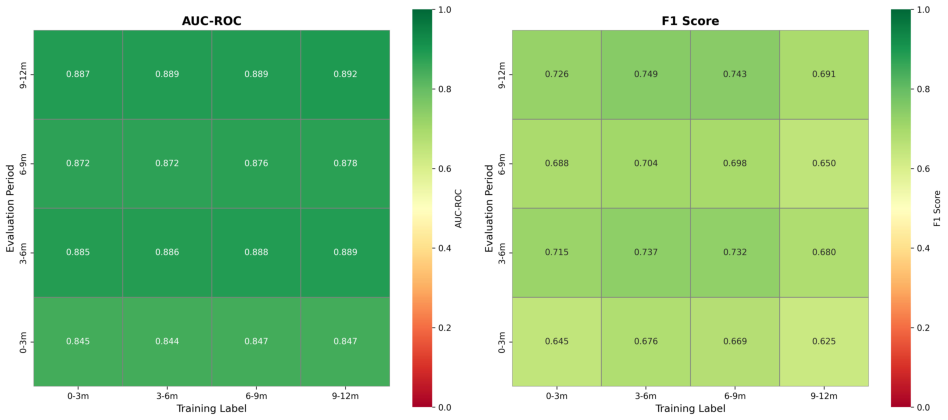
\includegraphics[width=0.8\linewidth]{./Hashimoto_fig/heatmap_conbined.pdf}
    \caption{各モデルのクロス評価(左:AUC,右:Recall)}
    \label{fig:Approach}
\end{figure*}


\todo{学習期間,予測期間を3ヶ月単位でスライディングウィンドウで評価した表(ヒートマップも載せる?)}
\subsection{RQ3:推定された報酬関数において、長期貢献者の継続的なタスク受け入れに寄与する特徴量(動機)は何か?}
\todo{報酬関数から算出された各重みの大きさを記載)}

\subsection{妥当性の脅威}
\todo{}

\subsection{おわりに}
\todo{}

\begin{acknowledgment}
hogehoge
\end{acknowledgment}


\bibliographystyle{ipsjunsrt}
\bibliography{bibsample}



\end{document}
